%% LaTeX2e class for student theses
%% sections/preliminary.tex
%% 
%% Karlsruhe Institute of Technology
%% Institute for Program Structures and Data Organization
%% Chair for Software Design and Quality (SDQ)
%%
%% Dr.-Ing. Erik Burger
%% burger@kit.edu
%%
%% Version 1.1, 2014-11-21


\chapter{Preliminary Definitions}
\label{ch:Preliminary}

In the following chapter we want to give the definitions of some of the 
\section{Introducing Cyber-Physical-Systems}
\label{sec:pre:cps}

In this thesis we take a close look at \textbf{CPS}. These are systems in which a physical aspect or value is controlled by a computer (program). For example, an aircraft control system in which the computer exerts a form of speed control on the airplane would be a CPS. 

In our case we take a closer look at the closely related notion of \textit{Hybrid Systems}, in which discrete values (in the control program) and continuous values (in the physical world) coexist. The difficulty in analyzing these kinds of systems stems from the ``hybridness'' of the systems: There is always some form of translation necessary to go from the program (discrete values) to the physical (continous reals) world. 

\subsection{Modelling CPS as Hybrid Automata}

Two different modelling approaches exist for CPS, the first one we now explain are hybrid automata. Formally they are defined to have the following components (cf. ~\cite{Heinzinger2000b}):
\begin{quote}
		\begin{description}
			\item[\textit{Variables}]A finite set \(X = \{x_1,\dots , x_n\}\) of real numbered variables. The number \(n\) is called the dimension of \(H\). [...]
			\item[\textit{Control graph}]A finite directed multigraph \((V, E)\). The vertices in \(V\) are called control modes. The edges in \(E\) are called control switches.
			\item[\textit{Initial, invariant, and flow conditions.}]Three vertex labeling functions \(init\), \(inv\) and \(flow\) that assign to each control mode \(v\in V\) three predicates. [...]
			\item[\textit{Jump conditions}]An Edge labeling function jump that assigns to each control switch  \(e \in E\) a predicate.
			\item[\textit{Events}]A finite set \(\Sigma\) of events, and an edge labeling function event: \(E \rightarrow \Sigma\) that assigns to each control switch an event.
		\end{description}
\end{quote} 

Based on non-deterministic finite automata (NFA), they are easy to understand for humans and serve well to model the abstract behavior of hybrid systems. A possible hybrid automata could look like in Fig.~\ref{fig:automata}.

\begin{figure}[ht!]
	\centering
	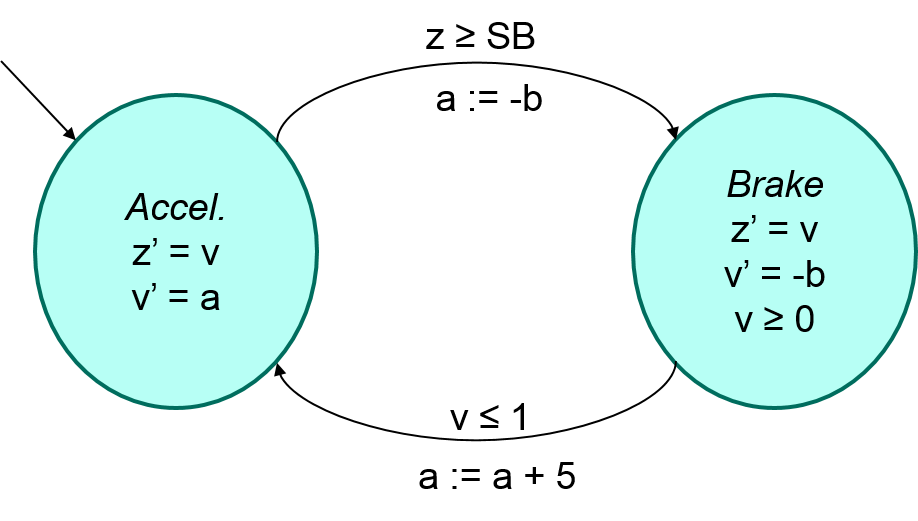
\includegraphics[width=1.0\textwidth]{images/automata}
	\caption{A simple Hybrid Automata~\cite{platze2010b}.}
	\label{fig:automata}
\end{figure}

\subsection{Modelling CPS as Hybrid Programs}

As we are using \keym~for verification, which uses Hybrid Programs, we also have to introduce the syntax of hybrid programs. They follow the syntax depicted in table~\ref{tab:hp}, whereby \(\theta_i\) are terms, \(x_i \in \Sigma\) are state variables and \(\chi\) is a formula of first-order logic~\cite{platzer2010b}.

As an example we take a look at the hybrid program notation of the ETCS example (See Fig.~\ref{fig:etcs_hp}). As can be seen, the state variable \(x\) is first assigned the state accelerate, this corresponds to the hybrid automaton's (See Fig.~\ref{fig:automata}) starting state of the system. In line 3 we can see the hybrid program syntax being an extension of first-order logic: Only if \(q=accel\) \textbf{and} \(z \geq SB\) are true can this case be enacted (corresponding to the state change from accel. to brake in the automaton).

\begin{table}
	\begin{tabular}{p{5cm} | p{4cm} | p{6cm} }
		notation & statement & effect \\ \hline
		\(x := \theta\) & discrete assignment & assigns term \(\theta\) to variable \(x\) \(\in\) \(V\) \\
		\(x := \ast\) & nondet. assignment & assigns any real value to \(x \in V\) \\
		\(x^{\prime}_1 = \theta_1 \wedge ... \newline
		... \wedge x^{\prime}_n = \theta_n \wedge \chi\) & continuous evolution & diff. equations for \(x_i \in V\) and terms \(\theta_i\),\newline
		with formula \(\chi\) as evolution domain \\
		\(?\chi\) & state check & test formula \(\chi\) at current state \\
		\(\alpha;\beta\) & seq. composition & HP \(\beta\) starts after HP \(\alpha\) finishes \\
		\(\alpha \cup \beta\) & nondet. choice & choice between alternatives HP \(\alpha\) or \(\beta\) \\
		\(\alpha^\ast\) & nondet. repetition & repeats HP \(\alpha\) \(n\)-times for any \(n \in \mathbb{N}\) \\
		\it{do} \(\alpha\) \it{until} \(\chi\) & evolve until &  evolve HP \(\alpha\) until \(\chi\) holds \\
	\end{tabular}
	\caption{Syntax of Hybrid Programs~\cite{platzer2010b}.}
	\label{tab:hp}
\end{table}

\begin{figure}[ht!]
	\(q := accel;\)\newline
	\(\cup~(?q = accel; z^{\prime}= v, v^{\prime}= a\) \newline
	\(\cup~(?q = accel \wedge z \geq SB; a := -b, q:= brake; ?v \geq 0)\) \newline
	\(\cup~(?q = brake; z^{\prime}=v, v^{\prime}= -b \wedge v \geq 0)\) \newline
	\(\cup~(?q = brake \wedge v \leq 1; a := a+5; q := accel))^\ast\)
	\caption{The simplified ETCS version as a Hybrid Program~\cite{platzer2010b}.}
	\label{fig:etcs_hp}
\end{figure}

\section{Dynamic Logic}
\label{sec:pre:DL}
